%%%%%%%%%%%%%%%%%%%%%%%%%%%%%%%%%%%%%%%%%%%%%%%%%%%%%%%%%
% LaTeX Beamer Presentation Generated by AI Researcher
% Paper: "Beyond Labels: Fine-Grained Detection and 
%         Explainable AI for Toxicity in Intimate Dialogues"
%%%%%%%%%%%%%%%%%%%%%%%%%%%%%%%%%%%%%%%%%%%%%%%%%%%%%%%%%

\documentclass[aspectratio=169]{beamer}

\usepackage[utf8]{inputenc}
\usepackage{amsmath}
\usepackage{amsfonts}
\usepackage{amssymb}
\usepackage{graphicx}
\usepackage{booktabs} % For professional tables
\usepackage{caption}  % Add this line for \captionof command

% Choose a theme
\usetheme{Madrid}
\usecolortheme{beaver}

% Adjustments for better presentation
\setbeamertemplate{navigation symbols}{} % Hide navigation symbols
\setbeamertemplate{footline}[frame number] % Show page number
\setbeamerfont{frametitle}{size=\large}
\setbeamerfont{title}{size=\huge}
\setbeamerfont{author}{size=\normalsize}
\setbeamerfont{institute}{size=\small}
\setbeamercovered{transparent} % Make covered items transparent

\title[Toxicity in Intimate Dialogues]{Beyond Labels: Fine-Grained Detection and Explainable AI for Toxicity in Intimate Dialogues}
\author{Nicolò Resta}
\institute{University of Bari, Aldo Moro}
\date{EVALITA 2025}

\begin{document}

% Title Slide
{
  \setbeamercolor{background canvas}{bg=white}
  \begin{frame}
    \titlepage
  \end{frame}
}

% Outline Slide
\begin{frame}
  \frametitle{Outline}
  \tableofcontents
\end{frame}

% --- SECTION 1: INTRODUCTION ---
\section{Introduction \& Motivation}

\begin{frame}
  \frametitle{The Challenge: Toxicity in Private Conversations}
  \begin{block}{The Problem}
        Detecting toxicity (harassment, abuse) is a critical NLP task for online safety.
        However, most research focuses on \textbf{public platforms} (e.g., Twitter, Reddit, Facebook, Instagram, Youtube).
      \end{block}
      
      \begin{alertblock}{Key Gaps in Private Dialogues}
        \begin{itemize}
          \item \textbf{Data Scarcity:} Sensitive, private nature makes data acquisition nearly impossible.
          \item \textbf{Context is Paramount:} Toxicity is subtle, dyadic, and depends on relational history.
          \item \textbf{Explainability is Crucial:} Simply flagging a chat as "toxic" is insufficient for trust and intervention. We need to answer questions like \textit{how much?} and \textit{why?}
        \end{itemize}
      \end{alertblock}
\end{frame}

\begin{frame}
  \frametitle{Our Contributions}
  
  \begin{enumerate}
    \item \textbf{A Novel Synthetic Data Generation Pipeline} \\
    % \pause
    We created a psychologically-grounded pipeline to generate realistic, dyadic \textbf{Italian chats}.
    \begin{itemize}
        \item Annotated with fine-grained, \textit{message-level continuous toxicity scores} [-1, 1].
        \item Includes \textit{human-readable narrative explanations} for chat dynamics.
    \end{itemize}
    \pause
    \item \textbf{A Comprehensive Empirical Study} \\
    % \pause
    We conducted experiments across three distinct tasks:
    \begin{itemize}
        \item Chat-Level Classification (Binary \& Multiclass)
        \item Message-Level Regression
        \item Abstractive Explanation Generation
    \end{itemize}
    \pause
    \item \textbf{A Rigorous Comparative Analysis} \\
    % \pause
    We statistically compared traditional ML models vs. transformer architectures, revealing key insights about the task's inherent limitations.
  \end{enumerate}
\end{frame}

\section{Dataset Preparation}

\begin{frame}
    \frametitle{A 3-Phase Synthetic Data Pipeline}
    \textbf{Phase 1, Personas Generation:}
    \begin{itemize}
        \item LLM acts as a psychologist.
        \item Creates detailed profiles: Big Five traits, Attachment styles, Emotional triggers, Personal history, And so on ...
    \end{itemize}
    \pause
    \textbf{Phase 2, Chat Generation:}
    \begin{itemize}
        \item Simulates chats across 7 relationship stages (e.g., infatuation, crisis).
        \item Controlled toxicity by targeting specific \textbf{mean} and \textbf{std. dev.} for message scores.
        \item Each message annotated with a polarity score in $[-1, 1]$.
    \end{itemize}
    \pause
    \textbf{Phase 3, Explanation Generation:}
    \begin{itemize}
        \item LLM acts as a communication expert.
        \item Generates a narrative rationale explaining the toxic or healthy dynamics of the entire chat.
    \end{itemize}

    \pause
    \begin{alertblock}{Result}
        A rich, nuanced dataset grounded in psychological plausibility, tailored for fine-grained analysis and explainability.
    \end{alertblock}
\end{frame}

\begin{frame}
  \frametitle{Dataset Filtering \& Labeling}
  
  \begin{block}{Final Dataset}
    After regex-parsing, filtering (e.g., max length 512 tokens) and cleaning (e.g. converting emojis to text), we obtained \textbf{1809} conversations.
  \end{block}

  \begin{block}{Labeling Scheme for Classification}
      \begin{itemize}
          \item \textbf{Continuous Message Scores} $\rightarrow$ \textbf{Discrete Chat Labels}.
          \item \textbf{Multiclass:}
          \begin{itemize}
              \item Toxic: $[-1, -0.35)$
              \item Neutral: $[-0.35, 0.35]$
              \item Healthy: $(0.35, 1]$
          \end{itemize}
          \item \textbf{Binary:} Toxic vs. Non-Toxic (Neutral + Healthy).
          \item \textbf{Aggregation:} Chat label is determined by the class of the \textit{minimum} user-average score.
      \end{itemize}
  \end{block}
\end{frame}

\begin{frame}
  \frametitle{Dataset Distribution}
  \centering
  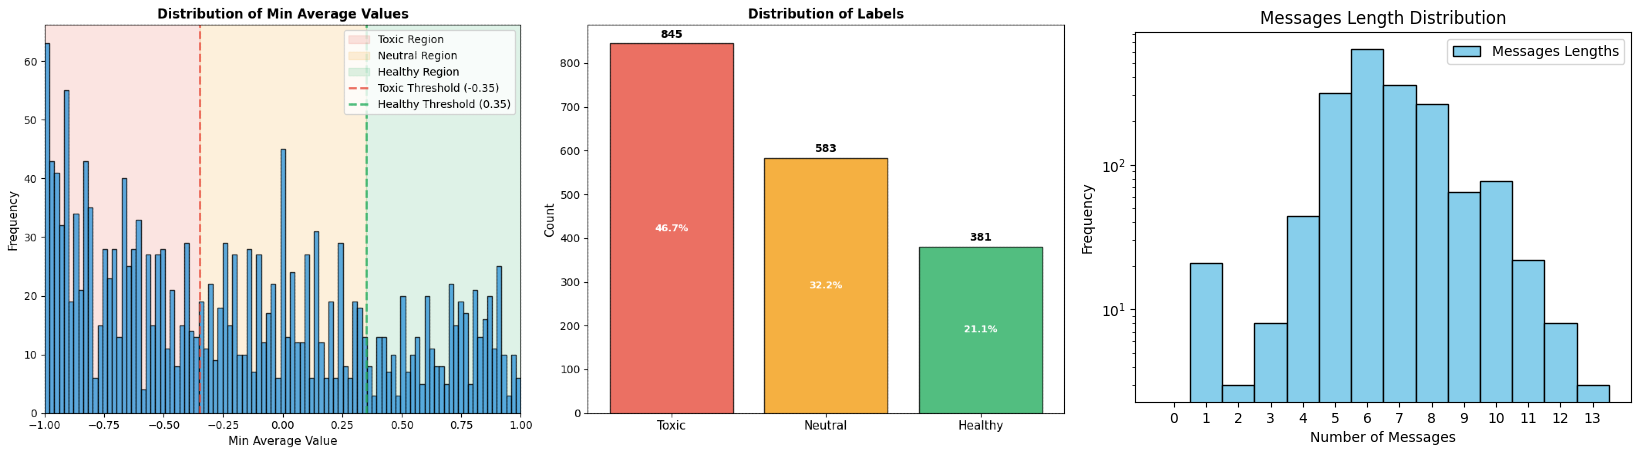
\includegraphics[width=\textwidth]{rsc/multiclass_distributions.png}
  % \captionof{figure}{Multiclass label distribution.}
\end{frame}

% --- SECTION 3: EXPERIMENTS ---
\section{Experiments}

\begin{frame}
  \frametitle{Models \& Tasks}
  
  \begin{columns}
    \begin{column}{0.5\textwidth}
      \begin{block}{1. Chat-Level Classification}
        \textbf{Classic Models:}
        \begin{itemize}
          \item Multinomial Naive Bayes (NB)
          \item Logistic Regression (LR)
          \item Support Vector Classifier (SVC)
        \end{itemize}
        \textbf{Transformer:}
        \begin{itemize}
          \item \texttt{dbmdz/bert-base-italian-cased}
        \end{itemize}
      \end{block}
    \end{column}
    \begin{column}{0.5\textwidth}
      \begin{block}{2. Message-Level Regression}
        \textbf{Transformer:}
        \begin{itemize}
          \item BERT to predict continuous message polarity scores.
        \end{itemize}
      \end{block}
      \begin{block}{3. Explanation Generation}
        \textbf{Transformer:}
        \begin{itemize}
          \item \texttt{morenolq/bart-it} to generate narrative explanations.
        \end{itemize}
      \end{block}
    \end{column}
  \end{columns}
\end{frame}

\begin{frame}
  \frametitle{Preprocessing \& Input Formatting}
  
  \textbf{Classic Models (LR, SVC, NB)}
    \begin{itemize}
      \item NLP Pipeline: Tokenization, POS filtering, NER-based anonymization.
      \item Normalization: Stemming vs. Lemmatization.
      \item Vectorization: CountVectorizer (NB) and TfidfVectorizer (LR, SVC).
    \end{itemize}
  
  \textbf{BERT Models}
    We explored various input strategies:
    \begin{itemize}
      \item \textbf{BERT (Classification):} Simple concatenation of all messages.
      \item \textbf{BERT-ST (Classification):} Separating speaker turns with `[SEP]` and using token-type IDs.
      \item \textbf{BERT-M (Regression):} Full chat as context, target message wrapped in `[SEP]`, distinguished with token-type IDs.
      \item \textbf{BERT-MU (Regression):} Role-aware variant of BERT-M with additional learned user embeddings.
    \end{itemize}
\end{frame}

\begin{frame}
  \frametitle{Rigorous Evaluation Protocol}
  
  \begin{alertblock}{Nested Cross-Validation}
    To get an unbiased performance estimate and tune hyperparameters simultaneously.
    \begin{itemize}
      \item \textbf{Outer Loop (5-fold):} For robust performance estimation.
      \item \textbf{Inner Loop (3-fold):} For hyperparameter tuning (\texttt{GridSearchCV}).
    \end{itemize}
  \end{alertblock}
  
  \begin{block}{Preventing Data Leakage}
    \textbf{\texttt{GroupKFold}} was used in both loops, ensuring all chats from the same couple remain in the same fold. This is crucial for valid results.
  \end{block}
  
  \begin{block}{Statistical Analysis}
    We computed means, stds, 95\% confidence intervals, and conducted \textbf{paired t-tests} on the outer fold scores to determine if performance differences were statistically significant.
  \end{block}
\end{frame}

% --- SECTION 4: RESULTS ---
\section{Results}

\begin{frame}
  \frametitle{Finding 1: A Performance Plateau in Classification}
  
  \begin{block}{Multiclass Classification (toxic, neutral, healthy)}
    \begin{itemize}
      \item Top models converge around a \textbf{Weighted F1-score of ~0.78}.
      \item \alert{Key Finding:} Classic models like \textbf{Logistic Regression} and \textbf{SVC} perform on par with more complex \textbf{BERT} architectures.
    \end{itemize}
  \end{block}
  
  \begin{columns}[T]
    \begin{column}{0.5\textwidth}
      \small
      \begin{tabular}{lcc}
        \toprule
        \textbf{Model} & \textbf{Weighted F1} & \textbf{Cost} \\
        \midrule
        PosNerStem-LR & $0.76 \pm 0.02$ & $0.11 \pm 0.01$ \\
        PosNerStem-SVC & $0.77 \pm 0.03$ & $0.11 \pm 0.01$ \\
        BERT & $0.77 \pm 0.03$ & $0.10 \pm 0.02$ \\
        \textbf{BERT-M (Reg.)} & $\mathbf{0.78 \pm 0.04}$ & $\mathbf{0.10 \pm 0.02}$ \\
        \bottomrule
      \end{tabular}
    \end{column}
    \begin{column}{0.5\textwidth}
      \centering
      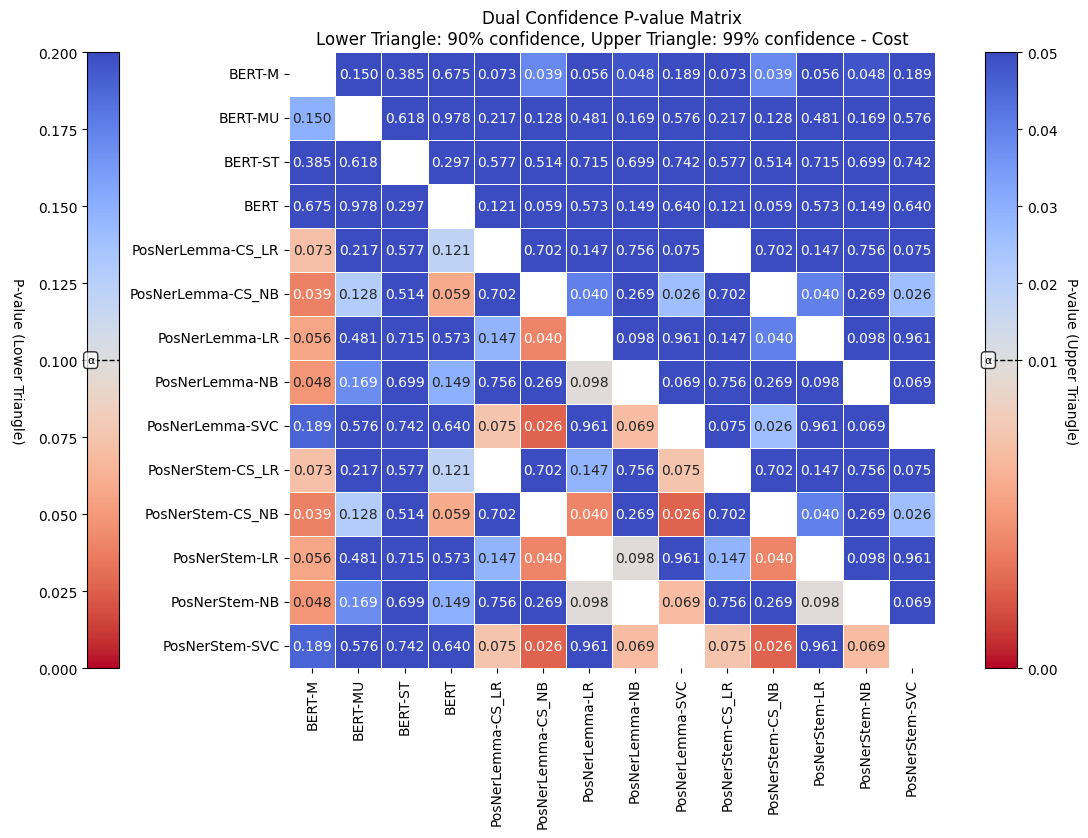
\includegraphics[width=\textwidth]{rsc/multiclass_statistical_tests2.png}
      \captionof{figure}{\small Paired t-tests show no significant difference among top models (blue = not significant).}
    \end{column}
  \end{columns}
  
  \begin{alertblock}{Interpretation}
    Performance is likely limited by the task's inherent \textbf{subjectivity and ambiguity}, not model complexity.
  \end{alertblock}
\end{frame}

\begin{frame}
    \frametitle{Finding 2: Regression is a Viable Alternative}
    
    \begin{block}{Message-Level Regression Performance}
        Both BERT regression models accurately predict continuous toxicity scores.
        \begin{itemize}
            \item \textbf{Correlation Coefficient > 0.82} with ground truth.
            \item Substantial improvement over a naive baseline (e.g., R-MAE ~0.46).
            \item The simpler \textbf{BERT-M} model slightly outperformed the role-aware \textbf{BERT-MU}.
        \end{itemize}
    \end{block}

    \begin{table}
        \centering
        \caption{Message-Level Regression Metrics}
        \small
        \begin{tabular}{lcc}
            \toprule
            \textbf{Metric} & \textbf{BERT-M} & \textbf{BERT-MU} \\
            \midrule
            Correlation Coefficient & $\mathbf{0.8335 \pm 0.0264}$ & $0.8254 \pm 0.0266$ \\
            Relative MAE (R-MAE) & $\mathbf{0.4618 \pm 0.0372}$ & $0.4687 \pm 0.0390$ \\
            \bottomrule
        \end{tabular}
    \end{table}

    \begin{alertblock}{Connecting Regression to Classification}
        When aggregating regression scores to produce chat-level labels, the \textbf{BERT-M} model achieves top-tier classification performance (\textbf{0.78 F1} multiclass, \textbf{0.87 F1} binary), proving the validity of the fine-grained approach. However, it does not offer a \textit{statistically significant} advantage over direct classification.
    \end{alertblock}
\end{frame}

\begin{frame}
  \frametitle{Finding 3: Promising Results in Explainability}
  
  \begin{block}{Abstractive Explanation Generation}
    The BART model was trained to generate narrative summaries of chat dynamics.
  \end{block}
  
  \begin{columns}[T]
    \begin{column}{0.5\textwidth}
      \begin{table}
        \centering
        \caption{Explanation Generation Test Metrics}
        \begin{tabular}{lr}
          \toprule
          \textbf{Metric} & \textbf{Value} \\
          \midrule
          \textbf{BERTScore (F1)} & \textbf{0.77} \\
          ROUGE-1 & 0.56 \\
          ROUGE-2 & 0.21 \\
          ROUGE-L & 0.25 \\
          BLEU & 0.20 \\
          \bottomrule
        \end{tabular}
      \end{table}
    \end{column}
    \begin{column}{0.5\textwidth}
      \begin{alertblock}{Interpretation}
        \begin{itemize}
            \item \textbf{High BERTScore F1 (0.77)} indicates strong \textit{semantic similarity} between generated and reference explanations. The model captures the correct meaning.
            \item Lower n-gram scores (ROUGE-2, BLEU) are expected in abstractive tasks with high linguistic variability.
            \item Overall: The model can generate coherent and contextually relevant rationales, a crucial step towards trustworthy AI.
        \end{itemize}
      \end{alertblock}
    \end{column}
  \end{columns}
\end{frame}


% --- SECTION 5: CONCLUSION ---
\section{Conclusion \& Future Work}

\begin{frame}
  \frametitle{Conclusions}
  
  \begin{itemize}
    \item We introduced a novel, psychologically-grounded pipeline for generating rich synthetic data for toxicity analysis in intimate dialogues.
    \pause
    \item Our key finding is a \textbf{performance plateau}: a diverse range of models (from LR to BERT) achieve statistically similar peak F1-scores (~0.78 multiclass, ~0.87 binary).
    \pause
    \item This suggests performance is currently bottlenecked by the \textbf{task's inherent ambiguity} and data characteristics, rather than model complexity.
    \pause
    \item The fine-grained regression approach is highly effective and performs competitively on classification tasks when its outputs are aggregated.
    \pause
    \item Our BART model demonstrates promising capabilities for generating \textbf{semantically relevant explanations}, paving the way for more transparent systems.
  \end{itemize}
\end{frame}

\begin{frame}
  \frametitle{Future Work}
  
  Our ongoing research focuses on four key areas:
  
  \begin{enumerate}
    \item \textbf{Enhancing Data Generation \& Quality Assessment} \\
    Refining the pipeline with automated quality metrics and exploring multi-agent (e.g., critic/generator) frameworks to improve realism.
    
    \item \textbf{Real-World Validation} \\
    Deploying a public demo to collect user feedback, bridging the "sim-to-real" gap and testing model generalization.
    
    \item \textbf{Multi-Task Learning for Enhanced Explainability} \\
    Training a single BART-based model for both regression and explanation generation, using explanation as a form of regularization to learn more robust representations.
    
    \item \textbf{Interdisciplinary Collaboration} \\
    Integrating professional psychologists into the research team to improve psychological fidelity and validate model behaviors.
  \end{enumerate}
\end{frame}

% Final Slide
\begin{frame}
  \centering
  \Huge Thank You! \\
  \vspace{0.5cm}
  \normalsize Questions?
\end{frame}

\end{document}